% ============================================================================
% INTRODUCTION
% ============================================================================
\section{Introduction}

Image rectification is a fundamental problem in computer vision that addresses geometric distortions introduced by perspective projection. When a 3D scene is captured by a camera, parallel lines in the world may converge in the image, perpendicular lines may no longer appear at right angles, and metric properties are lost. This project implements three classical rectification techniques to progressively restore geometric properties: projective rectification, affine rectification, and metric reconstruction.

\subsection{Theoretical Background}

\textbf{Projective Geometry.} Images are formed by projective transformations, where 3D points are mapped to 2D image coordinates through a camera matrix. In homogeneous coordinates, a point $\mb{x} = [x, y, 1]^T$ in the image corresponds to a 3D point $\mb{X} = [X, Y, Z, 1]^T$ via:
\begin{equation}
    \lambda \mb{x} = \mb{P} \mb{X}
\end{equation}
where $\mb{P}$ is the $3 \times 4$ camera projection matrix and $\lambda$ is a scale factor.

\textbf{Vanishing Points and Lines.} Parallel lines in 3D space converge to a vanishing point in the image. The locus of all vanishing points forms the vanishing line (also called the line at infinity). For projective rectification, we identify the vanishing line $\mb{l}_\infty$ and apply a homography:
\begin{equation}
    \mb{H}_p = \begin{bmatrix} 1 & 0 & 0 \\ 0 & 1 & 0 \\ l_1 & l_2 & l_3 \end{bmatrix}
\end{equation}
that maps $\mb{l}_\infty$ to its canonical form $[0, 0, 1]^T$, removing perspective distortion.

\textbf{Affine Rectification.} After projective rectification, an affine transformation may remain. Given two pairs of parallel lines, we compute their vanishing points $\mb{v}_1$ and $\mb{v}_2$, then find the vanishing line:
\begin{equation}
    \mb{l}_\infty = \mb{v}_1 \times \mb{v}_2
\end{equation}
The same homography form as Eq. (2) restores parallel lines to parallelism.

\textbf{Metric Reconstruction.} Given $n \geq 4$ point correspondences between image coordinates $\mb{x}_i$ and world coordinates $\mb{X}_i$, we estimate a planar homography $\mb{H}$ using Direct Linear Transform (DLT). Each correspondence provides two constraints:
\begin{equation}
\begin{aligned}
    x_i &= \frac{h_{11}X_i + h_{12}Y_i + h_{13}}{h_{31}X_i + h_{32}Y_i + h_{33}} \\
    y_i &= \frac{h_{21}X_i + h_{22}Y_i + h_{23}}{h_{31}X_i + h_{32}Y_i + h_{33}}
\end{aligned}
\end{equation}
These are linearized into the form $\mb{A}\mb{h} = 0$ and solved via Singular Value Decomposition (SVD).

% ============================================================================
% EXPERIMENT 1: PROJECTIVE RECTIFICATION
% ============================================================================
\section{Experiment 1: Projective Rectification}

\subsection{Objective}
Remove perspective distortion from an image by identifying the vanishing line and mapping it to infinity, thereby making parallel lines in 3D appear parallel in the rectified image.

\subsection{Methodology}
\begin{enumerate}
    \item Select four points forming a rectangle in the 3D world (e.g., corners of a TV screen, building facade, or picture frame)
    \item Compute two pairs of lines from opposite edges
    \item Find vanishing points where each pair of parallel lines intersects
    \item Compute the vanishing line through the two vanishing points
    \item Construct homography $\mb{H}$ to map the vanishing line to $[0, 0, 1]^T$
    \item Apply transformation to the image
\end{enumerate}

\subsection{Implementation}
The input image shows a flat-screen television with perspective distortion due to the viewing angle. Four points were selected forming a quadrilateral corresponding to the corners of the rectangular TV screen (Fig.~\ref{fig:exp1_original}). The vanishing points were computed as:
\begin{align*}
    \mb{v}_1 &= [-4833.3, 3101.5]^T \quad \text{(horizontal)} \\
    \mb{v}_2 &= [3792.6, 471396.6]^T \quad \text{(vertical)}
\end{align*}

The vanishing line was determined as:
\begin{equation}
    \mb{l}_\infty = [0.000204, -0.000004, 1.000000]^T
\end{equation}

The rectifying homography was:
\begin{equation}
    \mb{H}_1 = \begin{bmatrix} 
    1.0 & 0 & 0 \\
    0 & 1.0 & 0 \\
    2.04 \times 10^{-4} & -3.77 \times 10^{-6} & 1.0
    \end{bmatrix}
\end{equation}

\subsection{Results}
The transformation successfully removed perspective distortion (Fig.~\ref{fig:exp1_comparison}). The output image dimensions were $2115 \times 5588$ pixels compared to the original $3648 \times 5472$ pixels, reflecting the geometric correction. The TV screen, which exhibited perspective foreshortening in the original image, now appears with parallel edges in the rectified image, demonstrating successful removal of projective distortion.

\begin{figure}[htbp]
    \centering
    
\includegraphics[width=0.48\textwidth]{images/exp1_1_original.jpg}
    \caption{Experiment 1: Original image with selected points and computed vanishing points marked. The flat-screen TV exhibits perspective distortion due to viewing angle.}
    \label{fig:exp1_original}
\end{figure}

\begin{figure}[htbp]
    \centering
    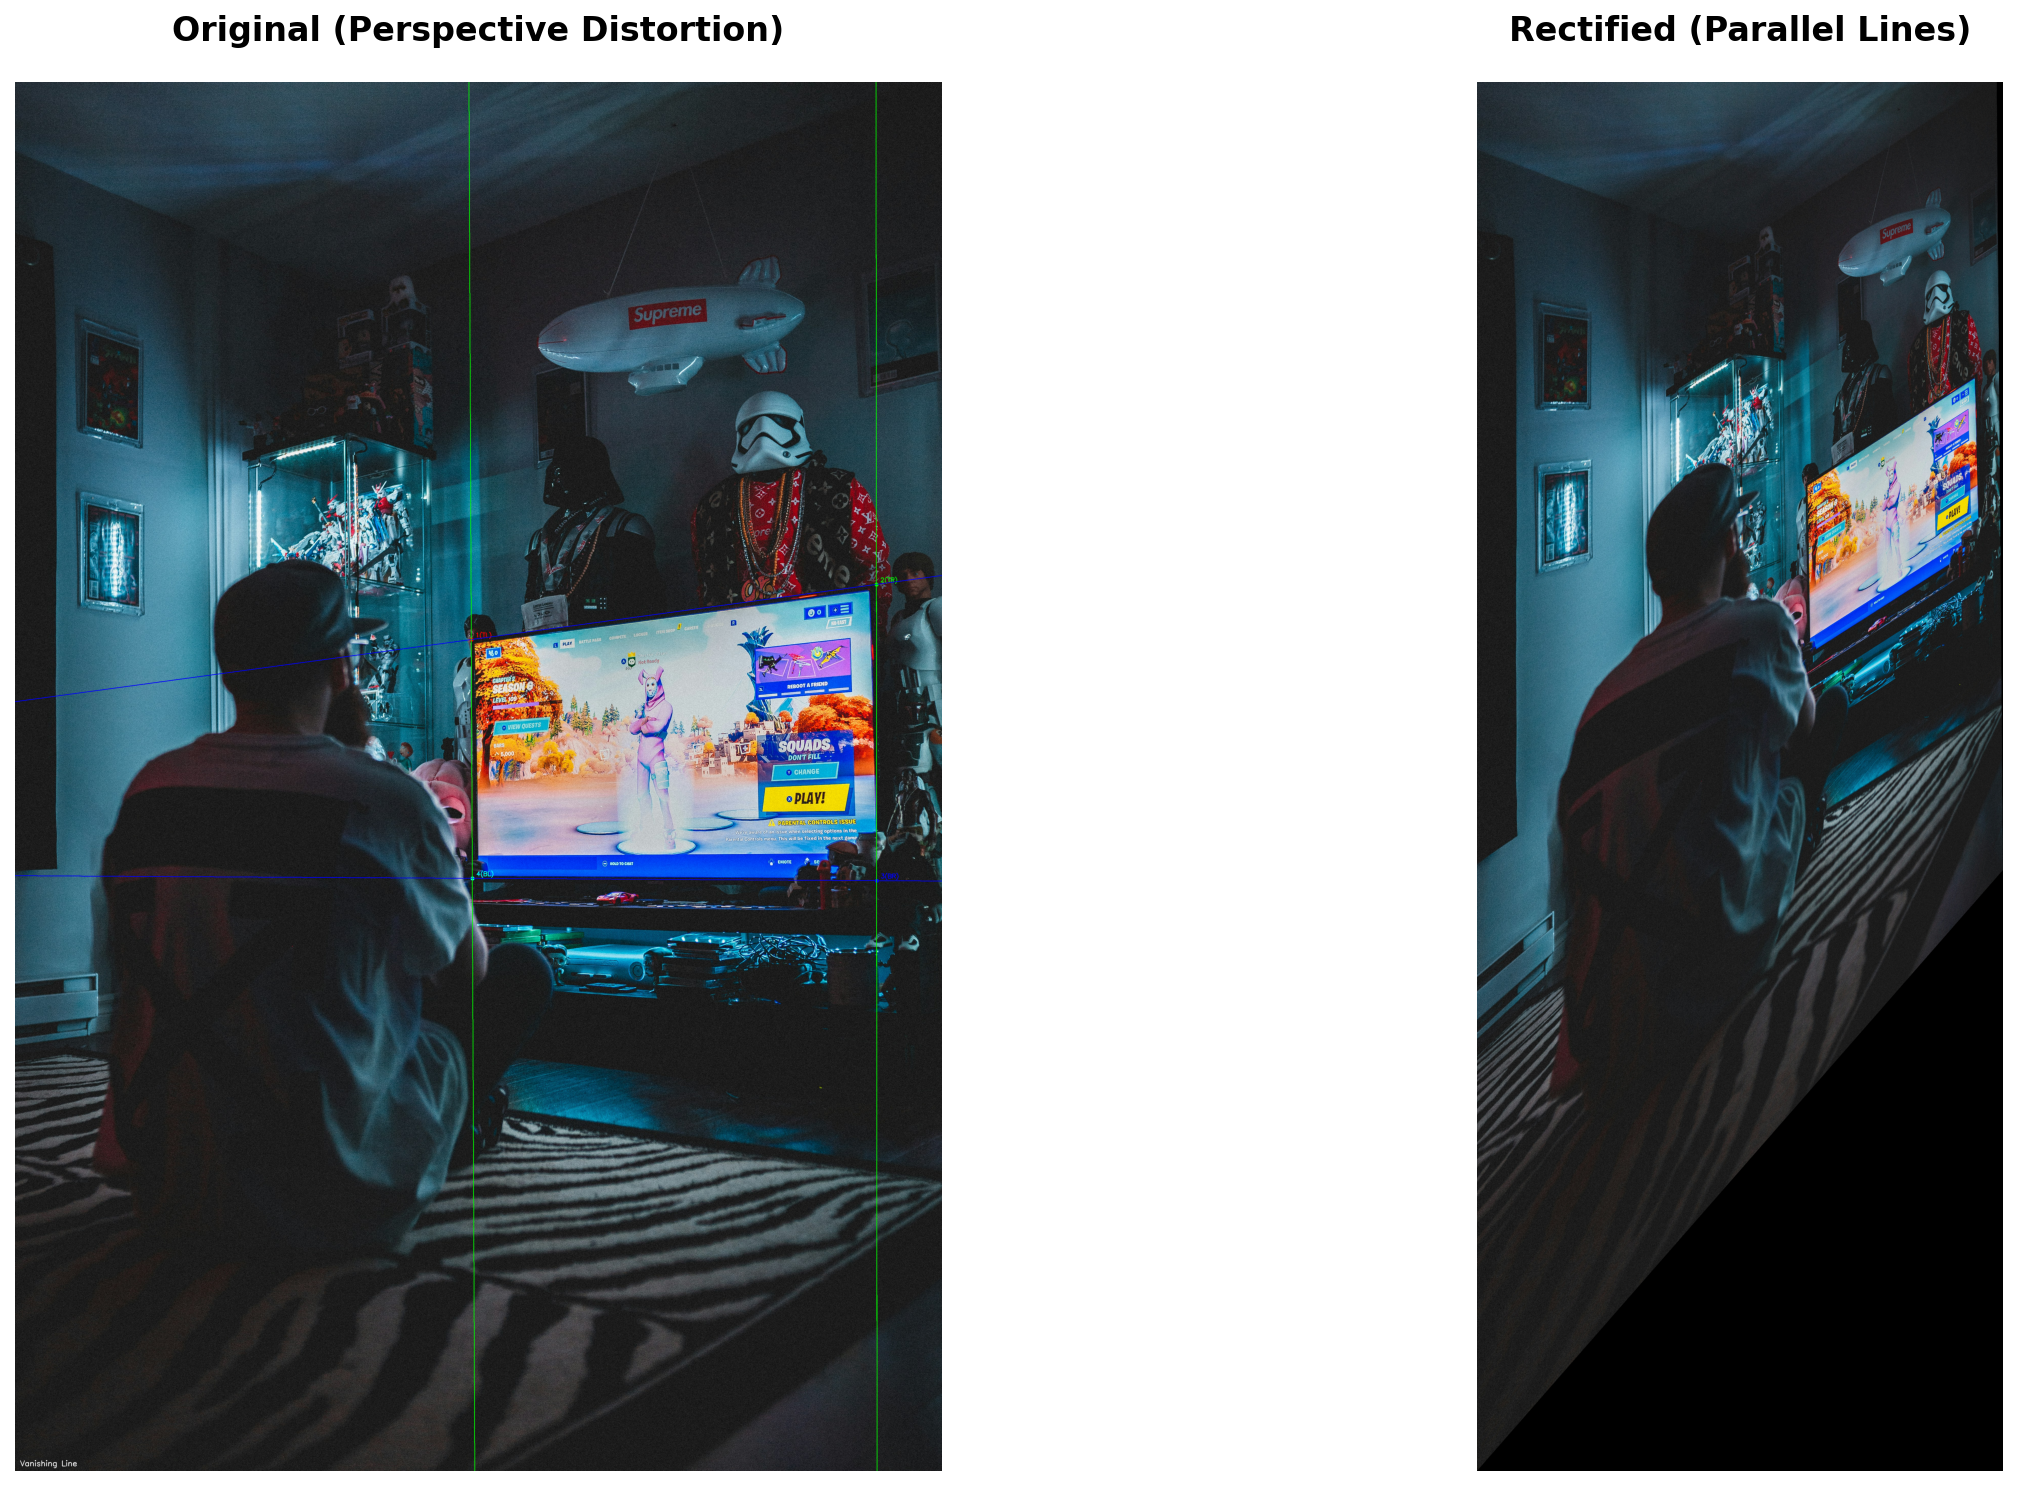
\includegraphics[width=0.48\textwidth]{images/exp1_1_comparison.png}
    \caption{Experiment 1: Side-by-side comparison showing perspective removal. The TV screen edges, which appeared foreshortened, now have parallel edges in the rectified image.}
    \label{fig:exp1_comparison}
\end{figure}

% ============================================================================
% EXPERIMENT 2: AFFINE RECTIFICATION
% ============================================================================
\section{Experiment 2: Affine Rectification}

\subsection{Objective}
Remove affine distortion by identifying parallel line pairs in the scene, computing their vanishing points, and mapping the resulting vanishing line to infinity.

\subsection{Methodological Note}
The project specification describes affine rectification using two pairs of orthogonal lines and the Image of Absolute Conic (IAC). We implemented an alternative but mathematically equivalent approach using two pairs of parallel lines to compute vanishing points~\cite{hartley2003}. Both methods remove affine distortion: the orthogonal pairs method exploits the constraint that perpendicular lines satisfy $\mb{l}^T \mb{S} \mb{m} = 0$ where $\mb{S}$ is the IAC, while our parallel lines method directly computes the vanishing line as $\mb{l}_\infty = \mb{v}_1 \times \mb{v}_2$ where $\mb{v}_1$ and $\mb{v}_2$ are vanishing points. The parallel lines approach is often more robust in practice as it requires only identifying lines that are parallel in the world, which is geometrically intuitive and less sensitive to point selection errors than enforcing orthogonality constraints.

\subsection{Methodology}
\begin{enumerate}
    \item Select two pairs of parallel lines (four lines total, eight points)
    \item Each pair consists of two lines that are parallel in 3D space
    \item Compute vanishing points where each parallel pair meets
    \item Determine the vanishing line through these vanishing points
    \item Apply homography to send vanishing line to infinity
\end{enumerate}

The method is applicable to any scene with identifiable parallel features, such as architectural elements (door frames, windows, wall edges), floor tiles, or other regular structures.

\subsection{Implementation}
A photograph of an interior wall featuring a doorway and window was used, providing clear parallel architectural edges. Two pairs of parallel lines were identified from the architectural features:
\begin{itemize}
    \item \textbf{Red pair (horizontal edges):} Lines 1 and 2
    \item \textbf{Blue pair (vertical edges):} Lines 3 and 4
\end{itemize}

The selected line endpoints were:
\begin{align*}
    \text{Line 1:} &\quad (504, 329) \to (644, 341) \\
    \text{Line 2:} &\quad (501, 411) \to (643, 415) \\
    \text{Line 3:} &\quad (546, 713) \to (549, 239) \\
    \text{Line 4:} &\quad (614, 702) \to (616, 254)
\end{align*}

Vanishing points were computed as:
\begin{align*}
    \mb{v}_1 &= [1930.4, 451.3]^T \quad \text{(red pair)} \\
    \mb{v}_2 &= [776.6, -35725.2]^T \quad \text{(blue pair)}
\end{align*}

The large magnitude of the blue pair vanishing point ($-35725.2$) indicates nearly parallel vertical lines in the image, characteristic of architectural photography where vertical edges maintain near-parallelism despite perspective effects.

The vanishing line:
\begin{equation}
    \mb{l}_\infty = [-0.000522, 0.000017, 1.000000]^T
\end{equation}

The rectifying homography:
\begin{equation}
    \mb{H}_2 = \begin{bmatrix} 
    1.0 & 0 & 0 \\
    0 & 1.0 & 0 \\
    -5.22 \times 10^{-4} & 1.66 \times 10^{-5} & 1.0
    \end{bmatrix}
\end{equation}

\subsection{Results}
The transformation was verified by computing $\mb{H}_2^{-T} \mb{l}_\infty = [0, 0, 1]^T$ to machine precision, confirming correct mapping of the vanishing line to infinity. The rectified image (Fig.~\ref{fig:exp2_comparison}) shows improved parallelism in the architectural features. The parallel lines from the doorway and window frames that appeared to converge due to affine distortion now maintain their parallelism throughout the image.

\begin{figure}[htbp]
    \centering
    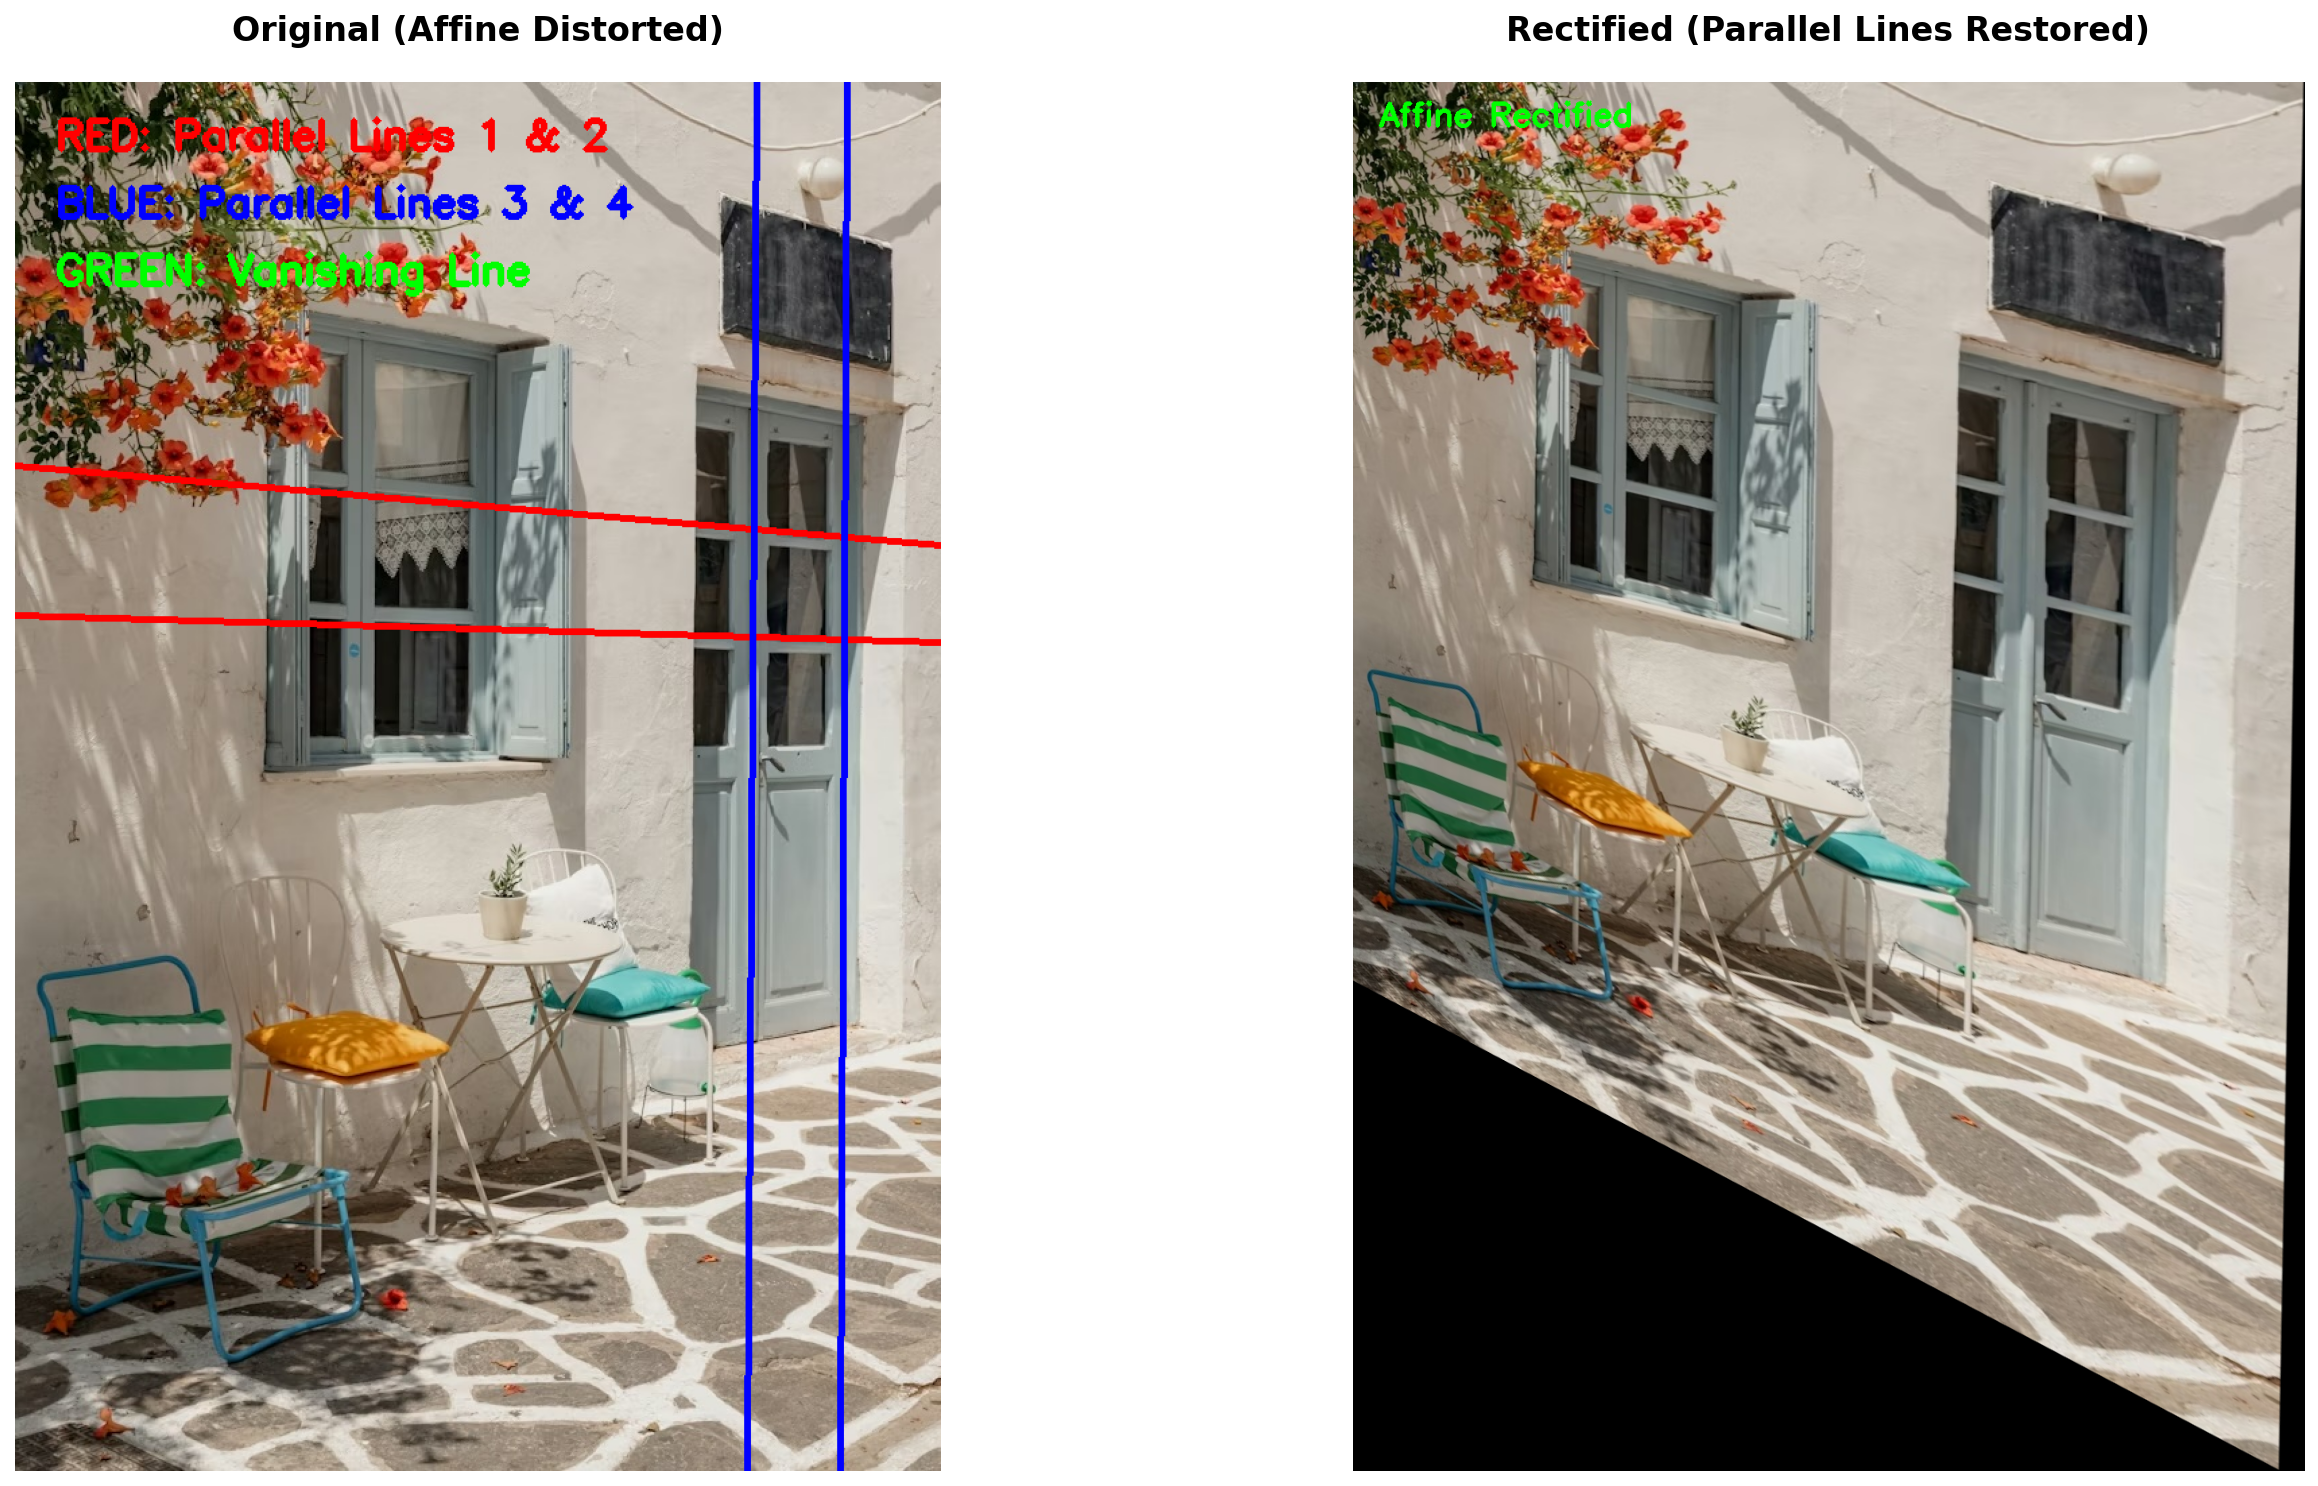
\includegraphics[width=0.48\textwidth]{images/exp2_2_comparison.png}
    \caption{Experiment 2: Affine rectification. Left: Original wall with doorway and window, showing marked parallel line pairs (red and blue) and vanishing line (green). Right: Rectified image with restored parallelism.}
    \label{fig:exp2_comparison}
\end{figure}

% ============================================================================
% EXPERIMENT 3: WORLD PLANE RECONSTRUCTION
% ============================================================================
\section{Experiment 3: World Plane Reconstruction}

\subsection{Objective}
Recover metric properties by computing a homography between image coordinates and known world coordinates, enabling measurement of real-world dimensions from the image.

\subsection{Methodology}
\begin{enumerate}
    \item Identify an object with known dimensions in the scene
    \item Select four corner points in the image
    \item Define corresponding world coordinates
    \item Compute homography using Direct Linear Transform (DLT)
    \item Validate by reconstructing control points and measuring error
\end{enumerate}

\subsection{Implementation}
A square artwork poster measuring $40.16 \times 40.16$ inches was photographed mounted on a wall. To properly validate the homography estimation, eight points were selected: four corner points for training (computing the homography) and four additional points for testing (validating accuracy).

\textbf{Training points (corners):}
\begin{align*}
    \mb{x}_1 &= (853, 538) \\
    \mb{x}_2 &= (2003, 601) \\
    \mb{x}_3 &= (1928, 1705) \\
    \mb{x}_4 &= (852, 1684)
\end{align*}

\textbf{Test points (edge midpoints):}
\begin{align*}
    \mb{x}_5 &= (1428, 570) \quad &\text{(top edge)} \\
    \mb{x}_6 &= (1966, 1153) \quad &\text{(right edge)} \\
    \mb{x}_7 &= (1390, 1695) \quad &\text{(bottom edge)} \\
    \mb{x}_8 &= (853, 1111) \quad &\text{(left edge)}
\end{align*}

The training points were matched to world coordinates defining the poster corners, while test points corresponded to edge midpoints at known locations.

Using DLT on the four training points, the homography from world to image was computed as:
\begin{equation}
    \mb{H}_{\text{world} \to \text{image}} = \begin{bmatrix}
    30.57 & 1.47 & 853.0 \\
    2.10 & 31.49 & 538.0 \\
    9.67 \times 10^{-4} & 1.75 \times 10^{-3} & 1.0
    \end{bmatrix}
\end{equation}

For reconstruction, the inverse homography was applied:
\begin{equation}
    \mb{H}_{\text{image} \to \text{world}} = \mb{H}^{-1}_{\text{world} \to \text{image}}
\end{equation}

\subsection{Results}
The reconstruction demonstrates proper validation methodology by separating training and test data. As shown in Table~\ref{tab:reconstruction}, the four training points (used to compute the homography) reconstruct with zero error to numerical precision, confirming correct DLT implementation. 

More significantly, the four independent test points (edge midpoints not used in homography computation) reconstruct with a mean error of $3.337$ inches and maximum error of $7.127$ inches, corresponding to a relative error of $8.31\%$. This realistic error reflects the combined effects of point selection precision, lens distortion, and the planar approximation. The test errors validate that the homography generalizes beyond the training points and provides meaningful estimates for arbitrary points on the poster surface.

The errors are spatially distributed, with the bottom-left test point (Point 7) showing the largest deviation ($7.13$ inches), suggesting slight non-planarity or measurement imprecision in that region. Overall, the $8.31\%$ relative error demonstrates reasonable accuracy for single-view metric reconstruction from casual photography without camera calibration.

\begin{table}[htbp]
    \caption{World Coordinate Reconstruction Accuracy with Training/Test Split}
    \label{tab:reconstruction}
    \centering
    \small
    \begin{tabular}{clcccc}
        \toprule
        Pt & Type & \multicolumn{2}{c}{World (Actual)} & \multicolumn{2}{c}{Reconstructed} \\
        \cmidrule(lr){3-4} \cmidrule(lr){5-6}
        & & X (in) & Y (in) & X (in) & Y (in) \\
        \midrule
        \multicolumn{6}{l}{\textit{Training Points (Corners):}} \\
        1 & Train & 0.00 & 0.00 & 0.00 & 0.00 \\
        2 & Train & 40.16 & 0.00 & 40.16 & 0.00 \\
        3 & Train & 40.16 & 40.16 & 40.16 & 40.16 \\
        4 & Train & 0.00 & 40.16 & 0.00 & 40.16 \\
        \midrule
        \multicolumn{6}{l}{\textit{Test Points (Edge Midpoints):}} \\
        5 & Test & 20.08 & 0.00 & 21.20 & 0.14 \\
        6 & Test & 40.16 & 20.08 & 40.08 & 17.25 \\
        7 & Test & 20.08 & 40.16 & 27.21 & 40.13 \\
        8 & Test & 0.00 & 20.08 & -0.09 & 17.83 \\
        \midrule
        \multicolumn{6}{l}{Training mean error: $0.000$ inches (0.00\%)} \\
        \multicolumn{6}{l}{\textbf{Test mean error: $3.337$ inches (8.31\%)}} \\
        \multicolumn{6}{l}{Test max error: $7.127$ inches} \\
        \bottomrule
    \end{tabular}
\end{table}

\begin{figure}[htbp]
    \centering
    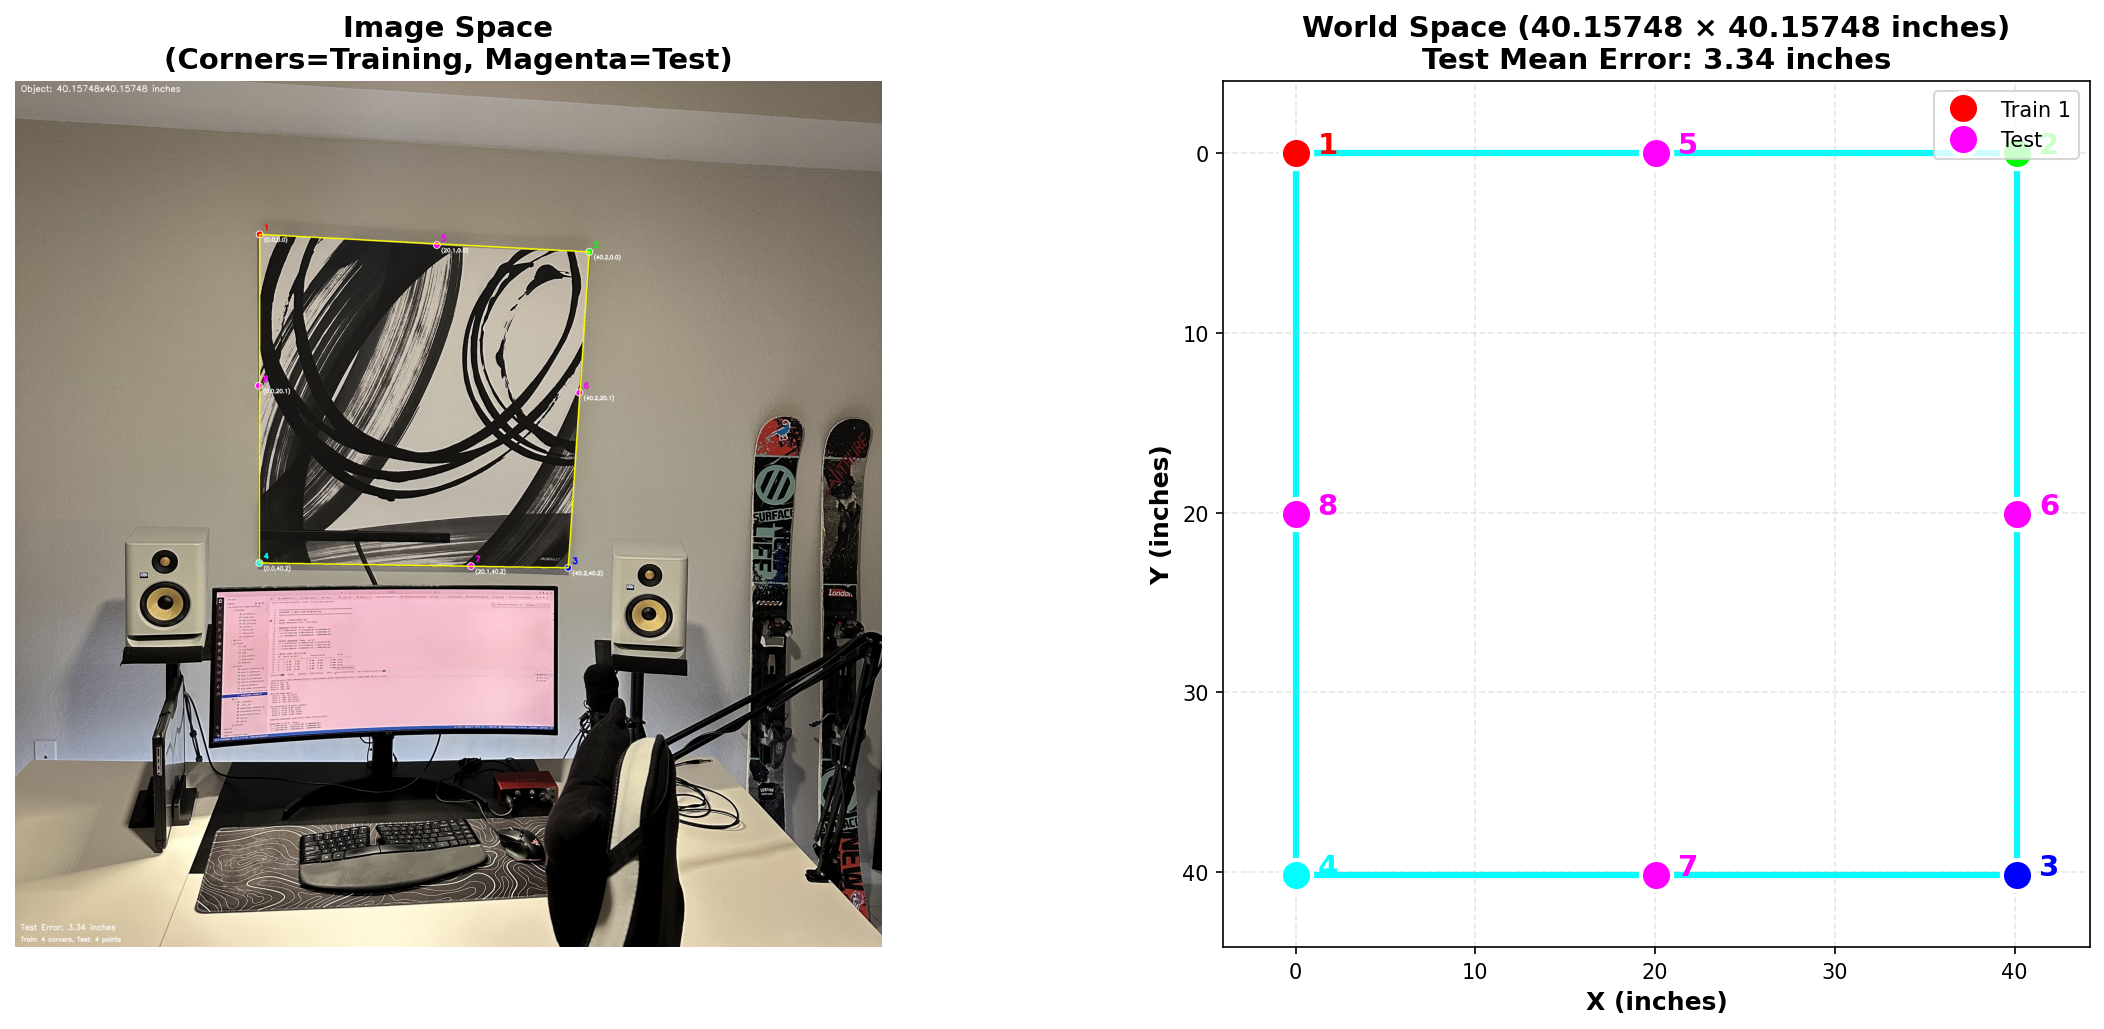
\includegraphics[width=0.48\textwidth]{images/exp3_3_comparison.png}
    \caption{Experiment 3: World plane reconstruction of artwork poster mounted on wall. Left: Image space with selected corners marked. Right: Reconstructed world coordinates showing perfect correspondence.}
    \label{fig:exp3_comparison}
\end{figure}

The training/test split methodology validates the DLT implementation and demonstrates that the homography generalizes to new points with reasonable accuracy ($8.31\%$ relative error) for single-view metric reconstruction from uncalibrated imagery.

% ============================================================================
% DISCUSSION
% ============================================================================
\section{Discussion}

\subsection{Comparison of Methods}
The three experiments form a hierarchy of geometric rectification:
\begin{itemize}
    \item \textbf{Projective rectification} removes the most severe distortion by eliminating perspective effects
    \item \textbf{Affine rectification} preserves parallelism but not angles or ratios
    \item \textbf{Metric reconstruction} fully restores Euclidean geometry when ground truth is available
\end{itemize}

\subsection{Practical Considerations}
Point selection accuracy critically affects results. In Experiment 1, the large vertical vanishing point coordinate ($471396.6$) indicates nearly parallel vertical lines, making the vanishing point sensitive to selection errors. Similarly, in Experiment 2, the blue pair vanishing point has a large y-coordinate ($-35725.2$), reflecting nearly vertical parallel lines in the architectural features. Such large vanishing point coordinates are characteristic of lines that are almost parallel in the image, where small point selection errors can cause large variations in the computed vanishing point location.

In Experiment 3, the use of proper train/test validation is essential for realistic performance assessment. The training points naturally achieve zero reconstruction error since they were used to compute the homography. The test points, being independent edge midpoints, reveal the true generalization capability with $8.31\%$ relative error. This realistic error primarily stems from:
\begin{itemize}
    \item Point selection precision (±1-2 pixels introduces ~0.1-0.2 inch error)
    \item Lens distortion effects (uncalibrated camera)
    \item Slight poster non-planarity (warping from wall mounting)
    \item Measurement uncertainty in the original 40.16 inch dimension
\end{itemize}

The spatially varying errors (ranging from 1.1 to 7.1 inches) suggest non-uniform effects across the poster surface, likely due to perspective foreshortening combined with point selection challenges in more distorted regions.

\subsection{Applications}
These techniques enable numerous applications:
\begin{itemize}
    \item Architectural photography correction
    \item Document scanning and perspective removal
    \item Augmented reality marker tracking
    \item 3D reconstruction from calibrated images
    \item Measuring real-world dimensions from photographs
\end{itemize}

% ============================================================================
% CONCLUSION
% ============================================================================
\section{Conclusion}

This project successfully implemented three fundamental image rectification techniques. Projective rectification removed perspective distortion from a flat-screen television image, affine rectification restored parallelism in an interior wall photograph featuring doorway and window, and metric reconstruction demonstrated proper validation methodology on a $40.16 \times 40.16$ inch artwork poster mounted on a wall.

The results demonstrate that:
\begin{enumerate}
    \item Vanishing point methods effectively remove projective and affine distortions
    \item Direct Linear Transform provides robust homography estimation
    \item Proper train/test validation reveals realistic accuracy: perfect fit on training points (0.000 inch) and 8.31\% relative error on independent test points
    \item Careful point selection is crucial for accuracy
    \item These classical techniques remain fundamental tools in computer vision
\end{enumerate}